\documentclass{beamer} 
\usepackage{amsmath,amsthm}
\usepackage{graphicx,microtype,parskip}
\usepackage{caption,subcaption,multirow}
\usepackage{attrib}
\usepackage{array}

\frenchspacing

\usetheme{default}
\usecolortheme{whale}

\setbeamertemplate{navigation symbols}{}

\setbeamercolor{title}{fg=blue,bg=white}

\setbeamercolor{block title}{fg=white,bg=gray}
\setbeamercolor{block body}{fg=black,bg=lightgray}

\setbeamercolor{block title alerted}{fg=white,bg=darkgray}
\setbeamercolor{block body alerted}{fg=black,bg=lightgray}


\title{How predictable is extinction?} 
\subtitle{Forecasting species survival at million-year timescales}
\author{Peter D Smits, Seth Finnegan}
\institute{Department of Integrative Biology, University of California -- Berkeley}
\date{}


\begin{document}


\begin{frame}
  \maketitle
\end{frame}


\begin{frame}
  \frametitle{Foundational assertion of conservation paleobiology }

  \begin{center}
    \begin{LARGE}
      By studying the \alert{past}, \\we can better predict the \alert{future}.
    \end{LARGE}
  \end{center}

\end{frame}


\begin{frame}
  \frametitle{What are we predicting?}

  \begin{center}
    \begin{LARGE}
      Extinction is \alert{hard} to predict, but is \alert{important} to conservation decisions.
    \end{LARGE}
  \end{center}

\end{frame}


\begin{frame}
  \frametitle{Predicting extinction}

  \begin{itemize}[<+->]
    \item A taxon with a \alert{greater than average} global geographic range is likely to \alert{survive for longer} than a taxon with \alert{less than average} global geographic range.
    \item A taxon's global geographic range can change over time.
    \item What happens to extinction risk as a taxon changes geographic range? How is extinction risk impacted if that taxon's global geographic range has recently \alert{increased} or \alert{decreased}?
  \end{itemize}

\end{frame}


\begin{frame}
  \frametitle{Data being analyzed}

  \begin{columns}
    \begin{column}{0.5\textwidth}
      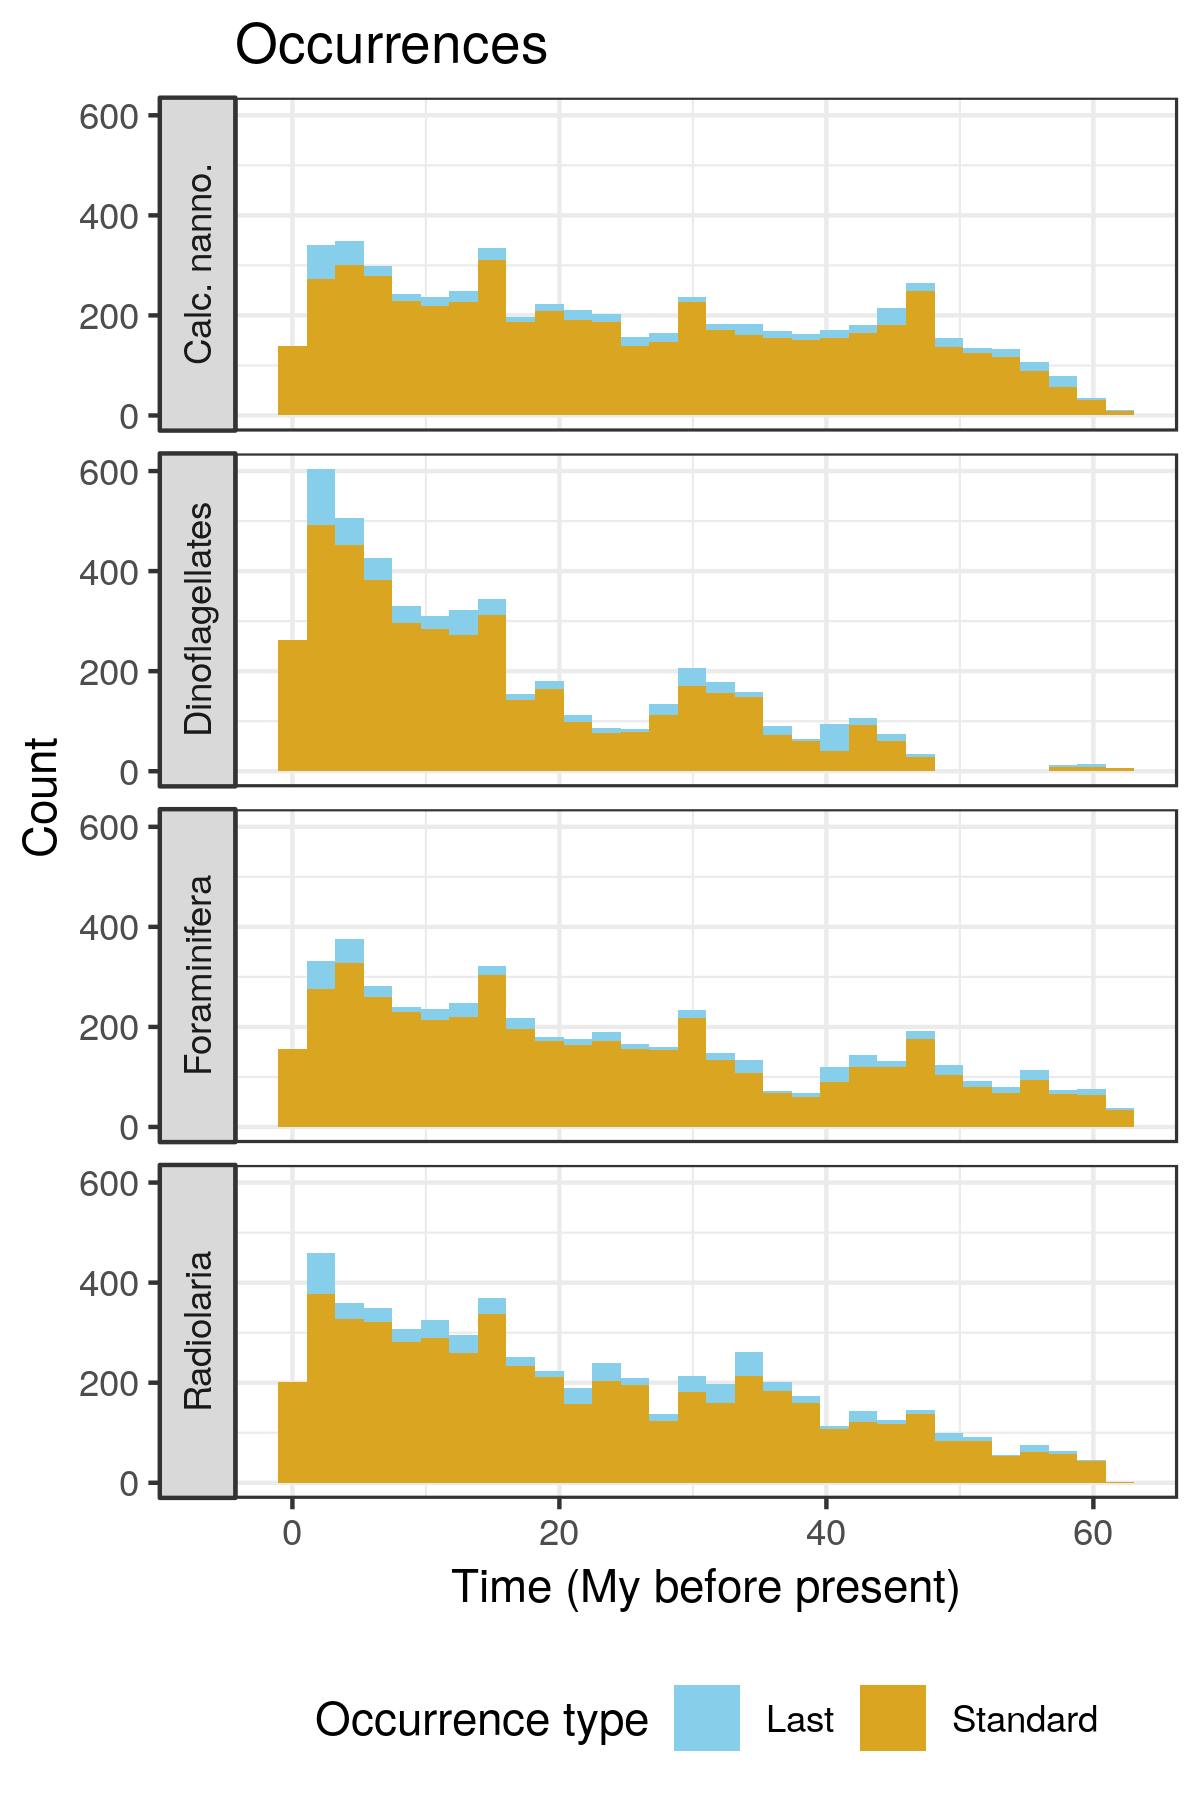
\includegraphics[width=\textwidth,height=0.8\textheight,keepaspectratio=true]{../results/figure/occ_time_label}
    \end{column}
    \begin{column}{0.5\textwidth}
      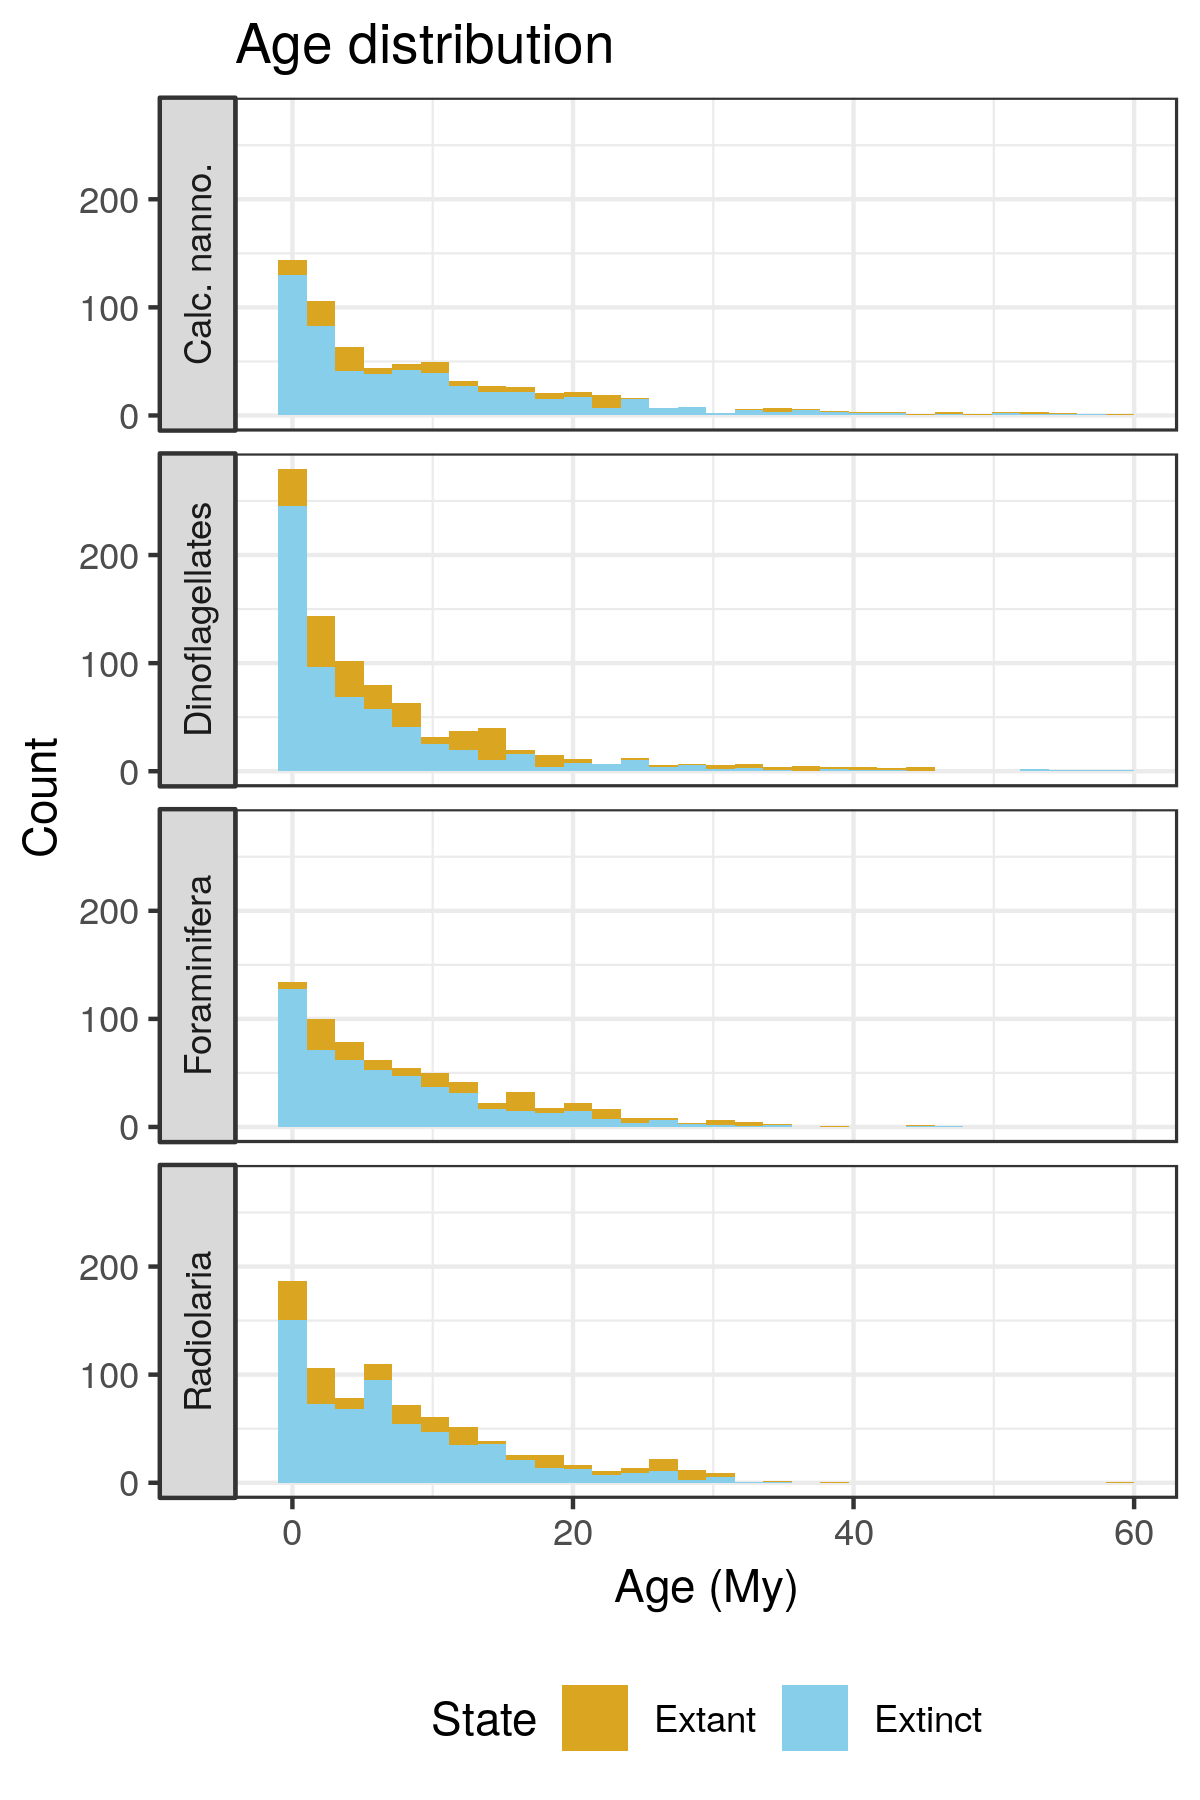
\includegraphics[width=\textwidth,height=0.8\textheight,keepaspectratio=true]{../results/figure/age_label}
    \end{column}
  \end{columns}

\end{frame}


\begin{frame}
  \frametitle{How we're analyzing the data}

  \begin{itemize}%[<+->]
    \item Encoding the past
      \begin{itemize}
        \item Change in geographic range between current observation and previous observation.
        \item Average global temperature at time of previous observation (Mg/Ca isotope).
        \item Age in millions of years at time of observation.
      \end{itemize}
    %\item \alert{Compare} models using WAIC/LOOIC.
    \item Explore model adequacy using posterior predictive distribution.
    \item Estimate out-of-sample predictive performance using \(k\)-fold cross-validation.
  \end{itemize}

\end{frame}


% explain ROC
% TYPES of errors
\begin{frame}
  \frametitle{Measuring performance: Reciever Operating Characteristic}

  \begin{center}
    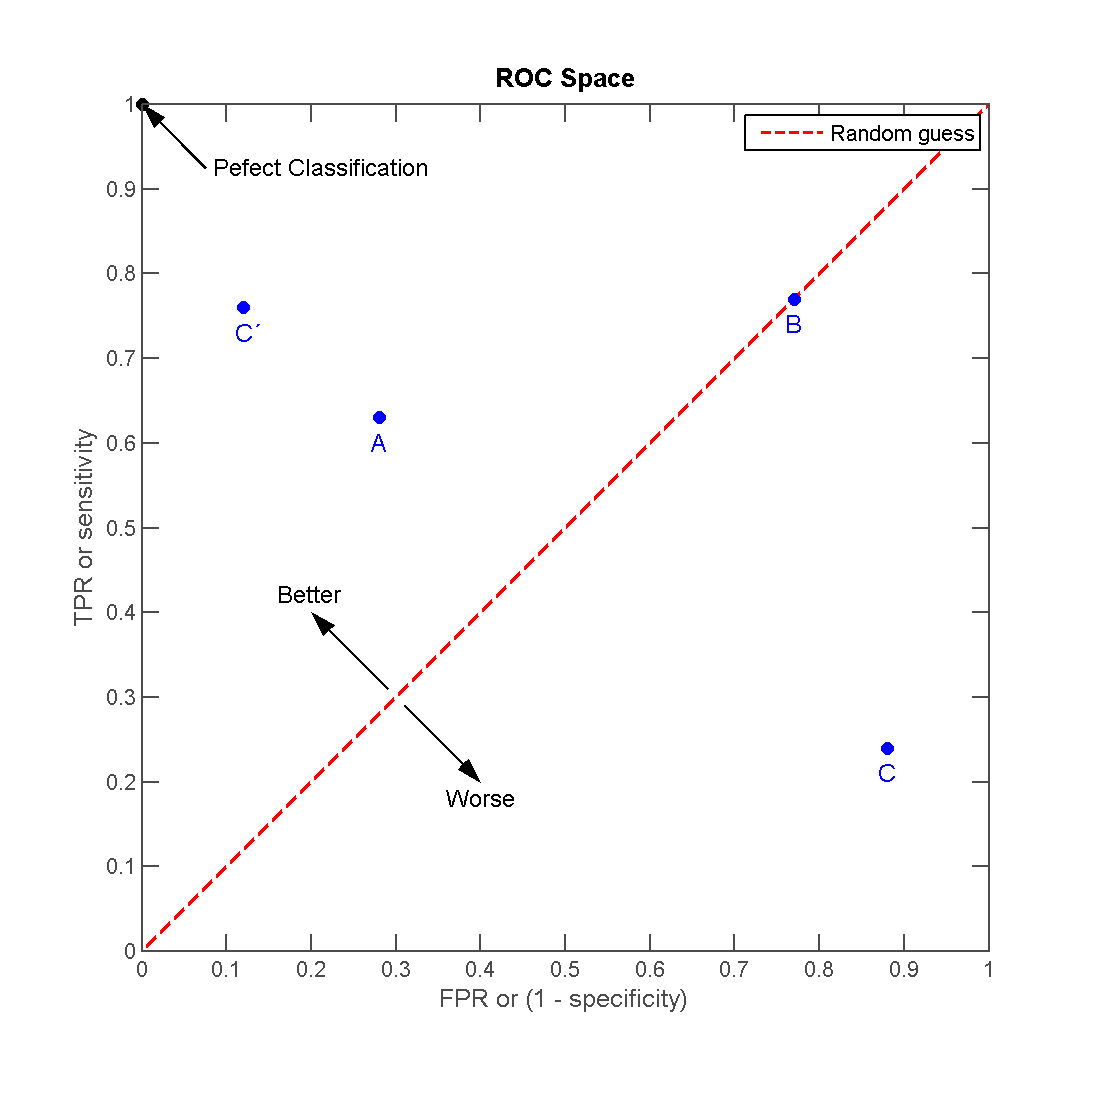
\includegraphics[width=\textwidth,height=0.8\textheight,keepaspectratio=true]{figure/wiki_ROC_space-2}
  \end{center}
  
  \attrib{\footnotesize{wikimedia}}

\end{frame}


\begin{frame}
  \frametitle{Measuring performance: Reciever Operating Characteristic}
  
  \begin{center}
    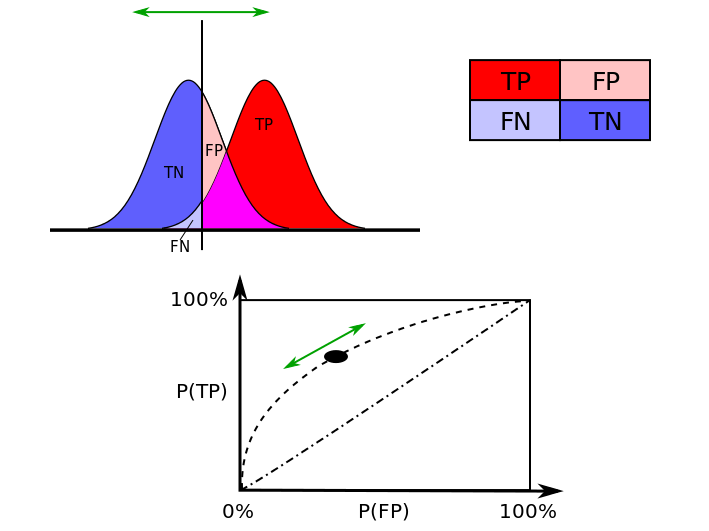
\includegraphics[width=\textwidth,height=0.8\textheight,keepaspectratio=true]{figure/wiki_709px-ROC_curves}
  \end{center}
  
  \attrib{\footnotesize{wikimedia}}
  
  % want to balance two rates: 
  %   true-positive rate -- predicting extinct when actual is extinct
  %   false-positive rate -- predicting extinct when actual is extant

  % curve describes these metrics at various thresholds

  % AUC is integral of ROC -- 0.5 is random classification, 1 is perfect classification
  
\end{frame}


\begin{frame}
  \frametitle{A conceptual model for predicting extinction}

\end{frame}


% demonstrate as ROC curve
\begin{frame}
  \frametitle{In-sample predictive performance, full dataset}

  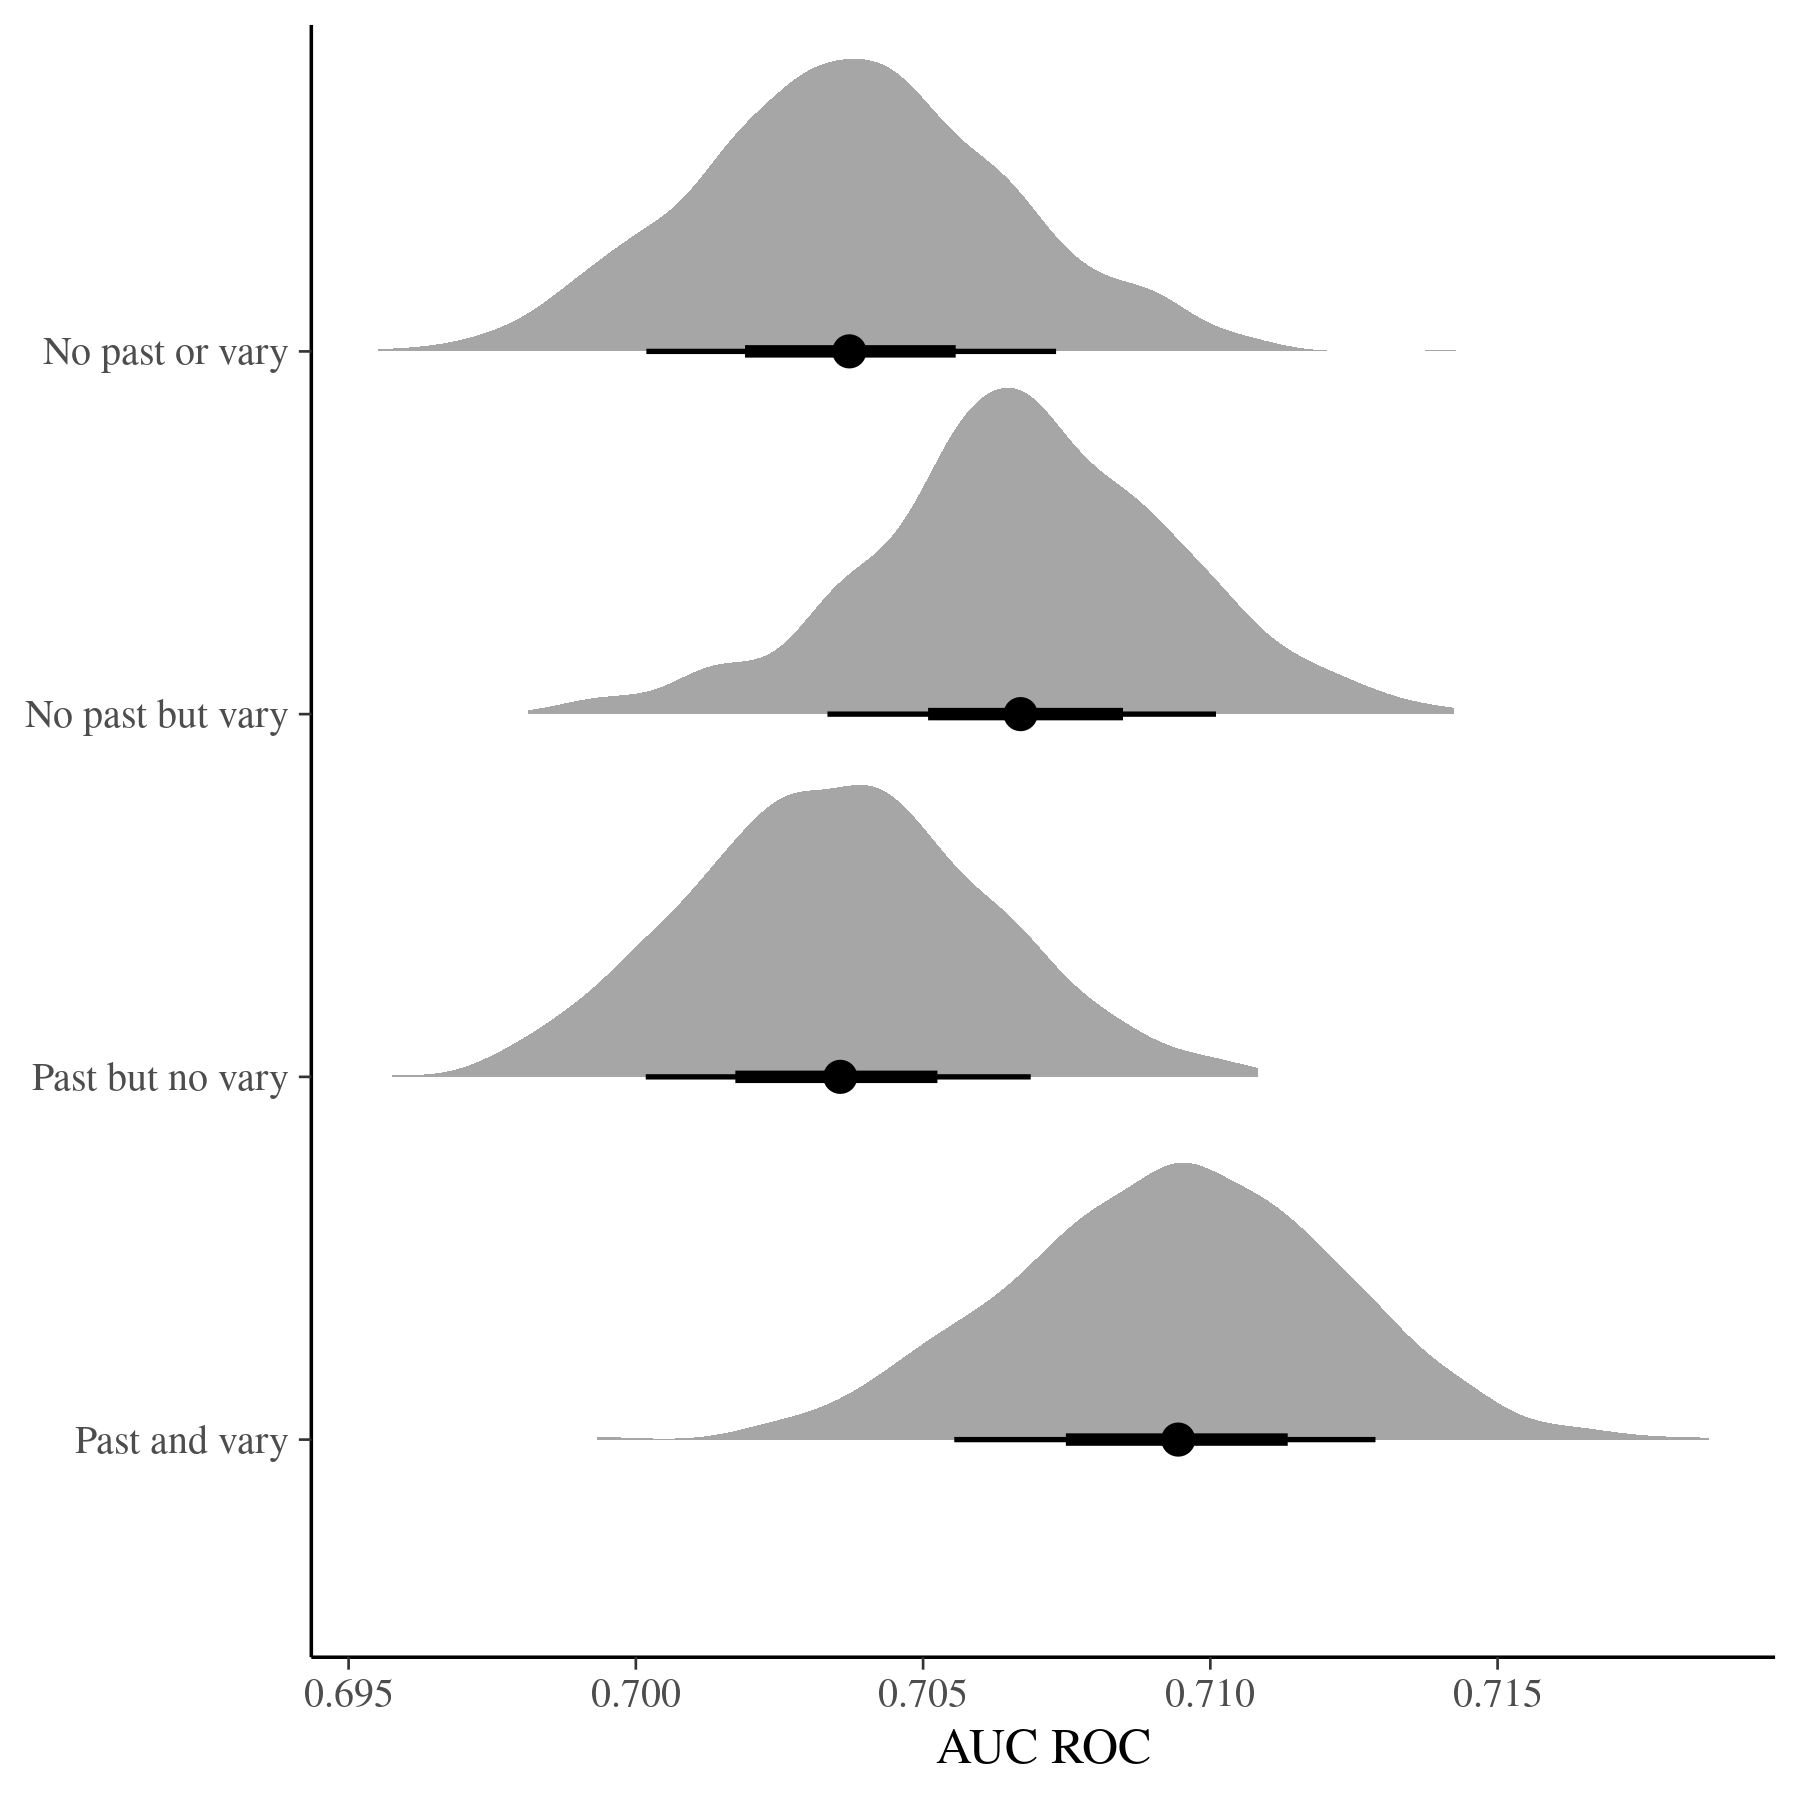
\includegraphics[width=\textwidth,height=0.8\textheight,keepaspectratio=true]{../results/figure/roc_hist}

\end{frame}


\begin{frame}
  \frametitle{In-sample predictive performance, by time}

  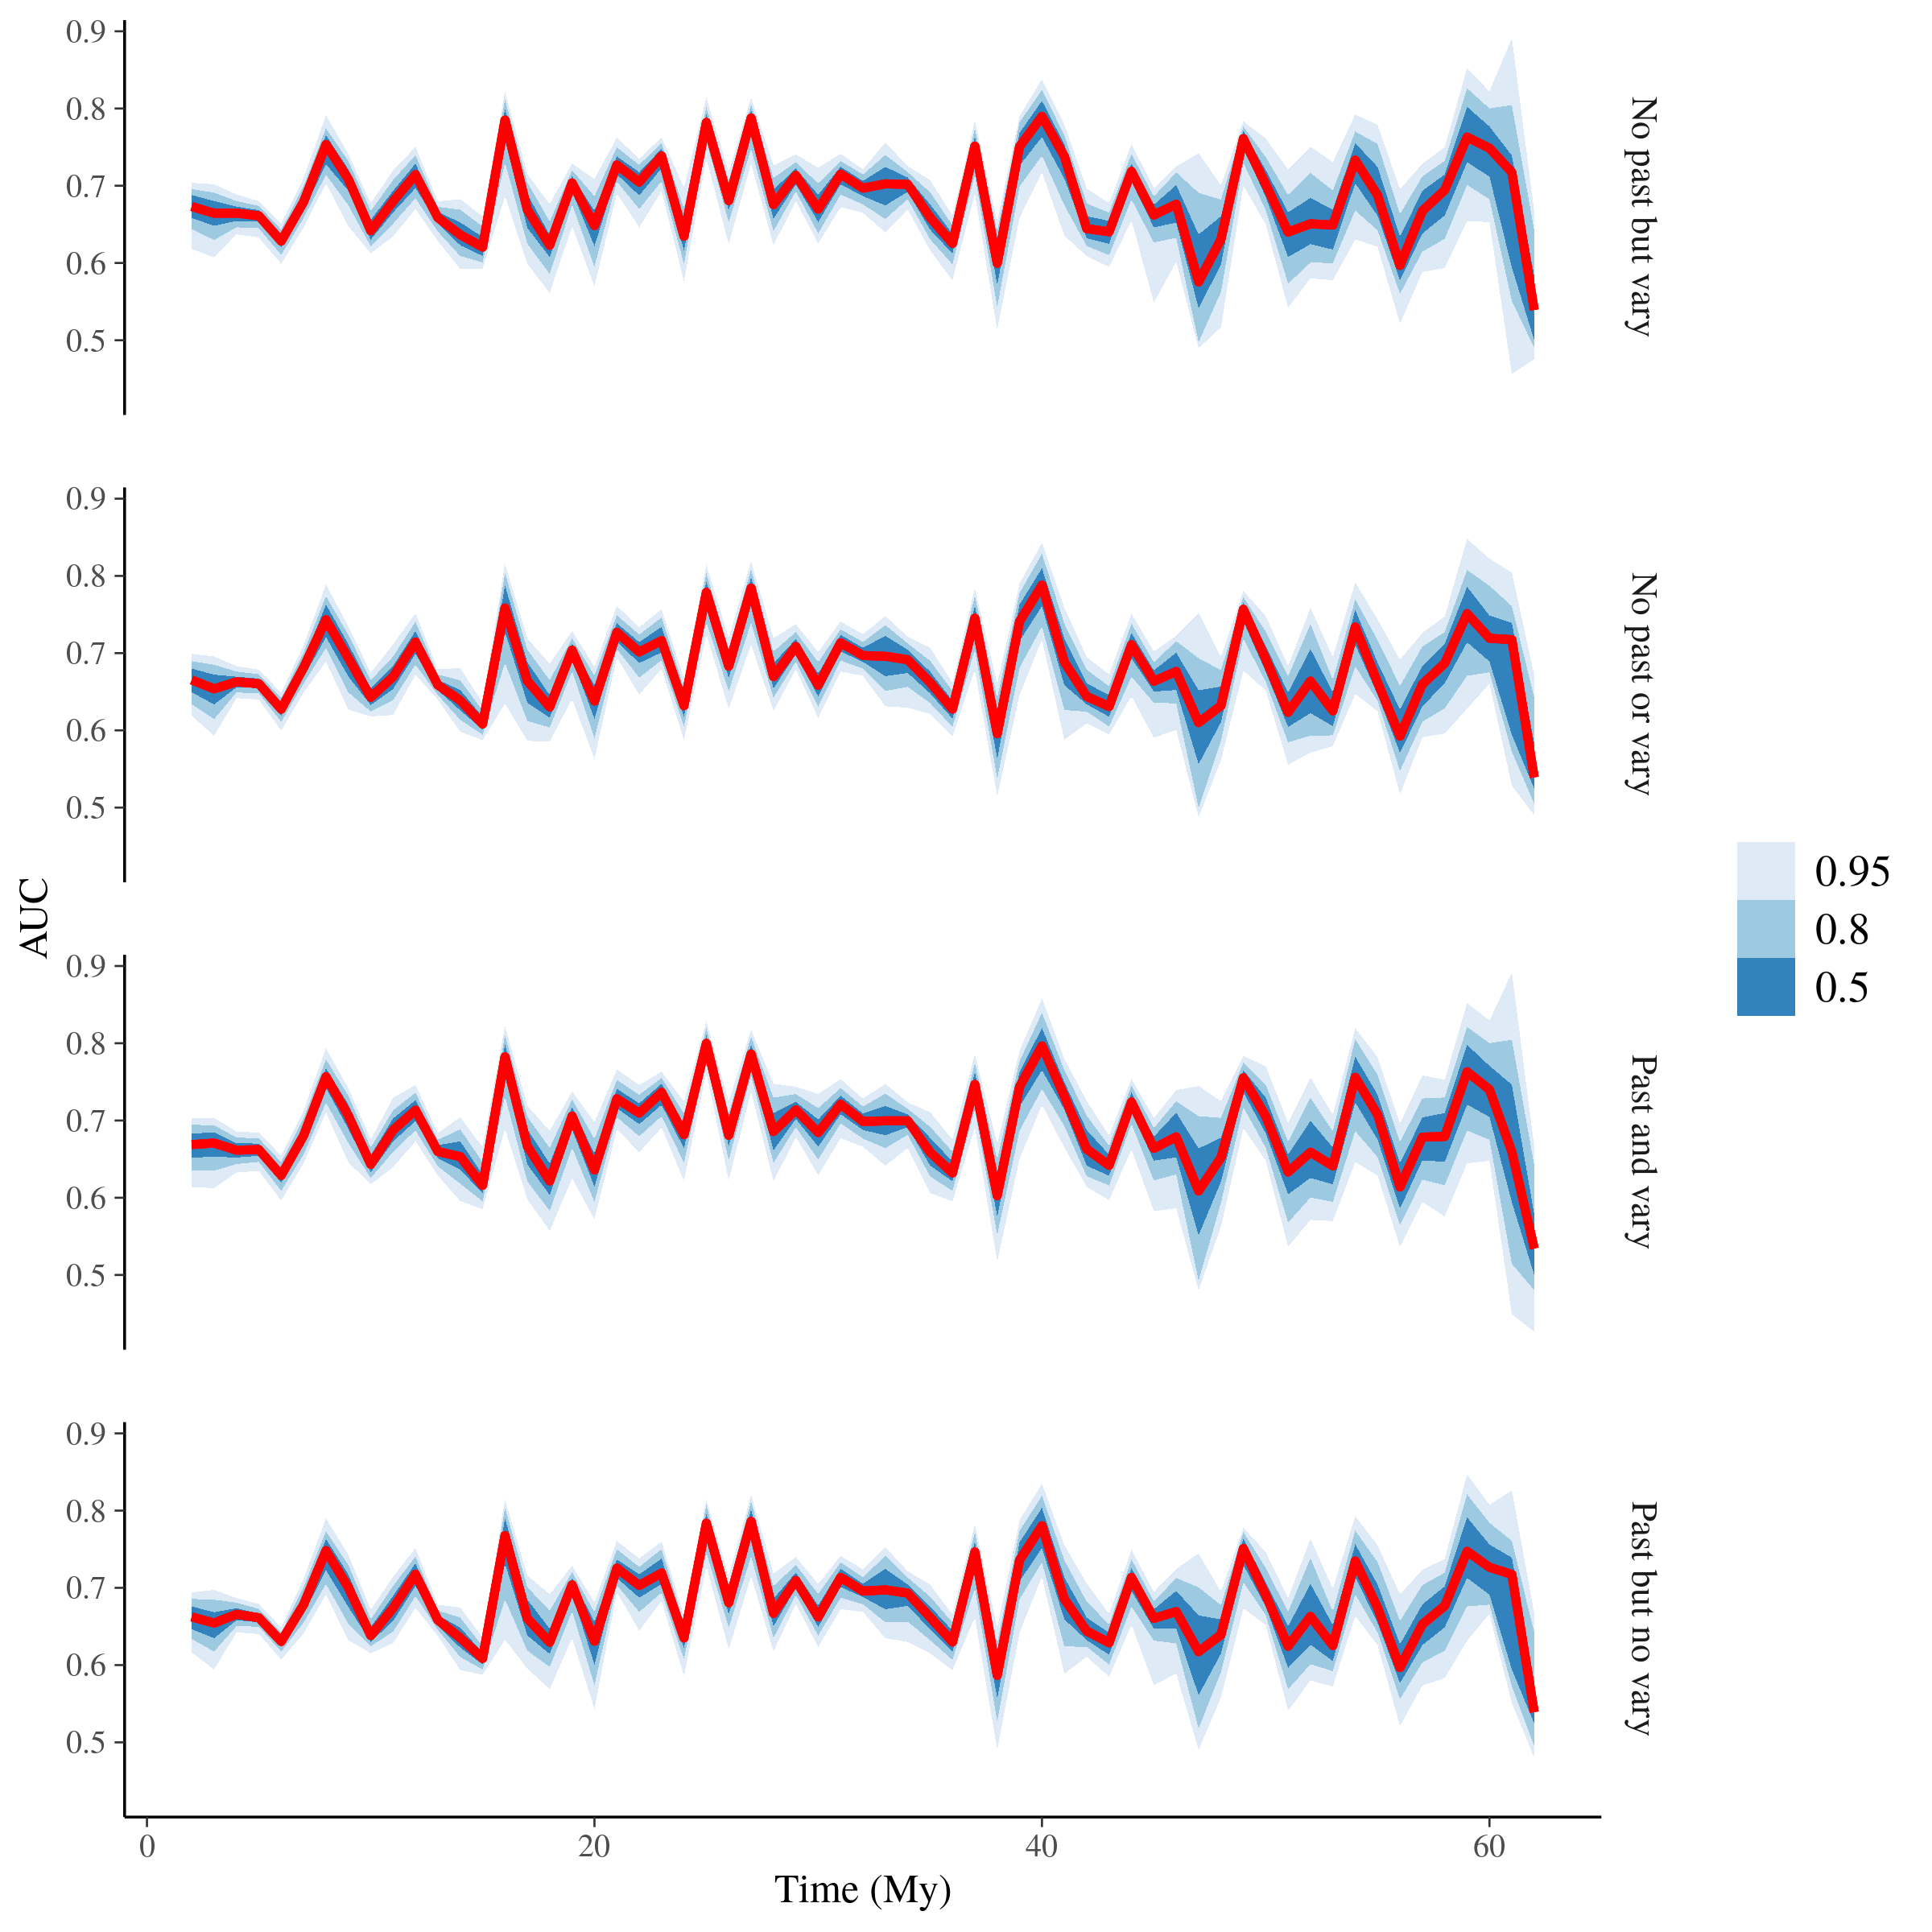
\includegraphics[width=\textwidth,height=0.8\textheight,keepaspectratio=true]{../results/figure/roc_ts}

\end{frame}


%% figure out way to present this graphically
%\begin{frame}
%  \frametitle{Comparing our models}
%
%  \begin{tabular}{ r c c c c }
%    Model & LOOIC & SE LOOIC & WAIC & SE WAIC \\ 
%    \hline
%    Past and vary & 12790.39 & \alert<2>{178.83} & 12786.06 & \alert<2>{178.77} \\ 
%    No past but vary & 12818.43 & \alert<2>{178.76} & 12815.40 & \alert<2>{178.71} \\ 
%    Past but no vary & 12850.45 & \alert<2>{179.42} & 12848.12 & \alert<2>{179.38} \\ 
%    No past or vary & 12850.87 & \alert<2>{179.46} & 12848.50 & \alert<2>{179.42} \\ 
%    \hline
%  \end{tabular}
%
%\end{frame}


\begin{frame}
  \frametitle{Cross-validation results, full dataset}

  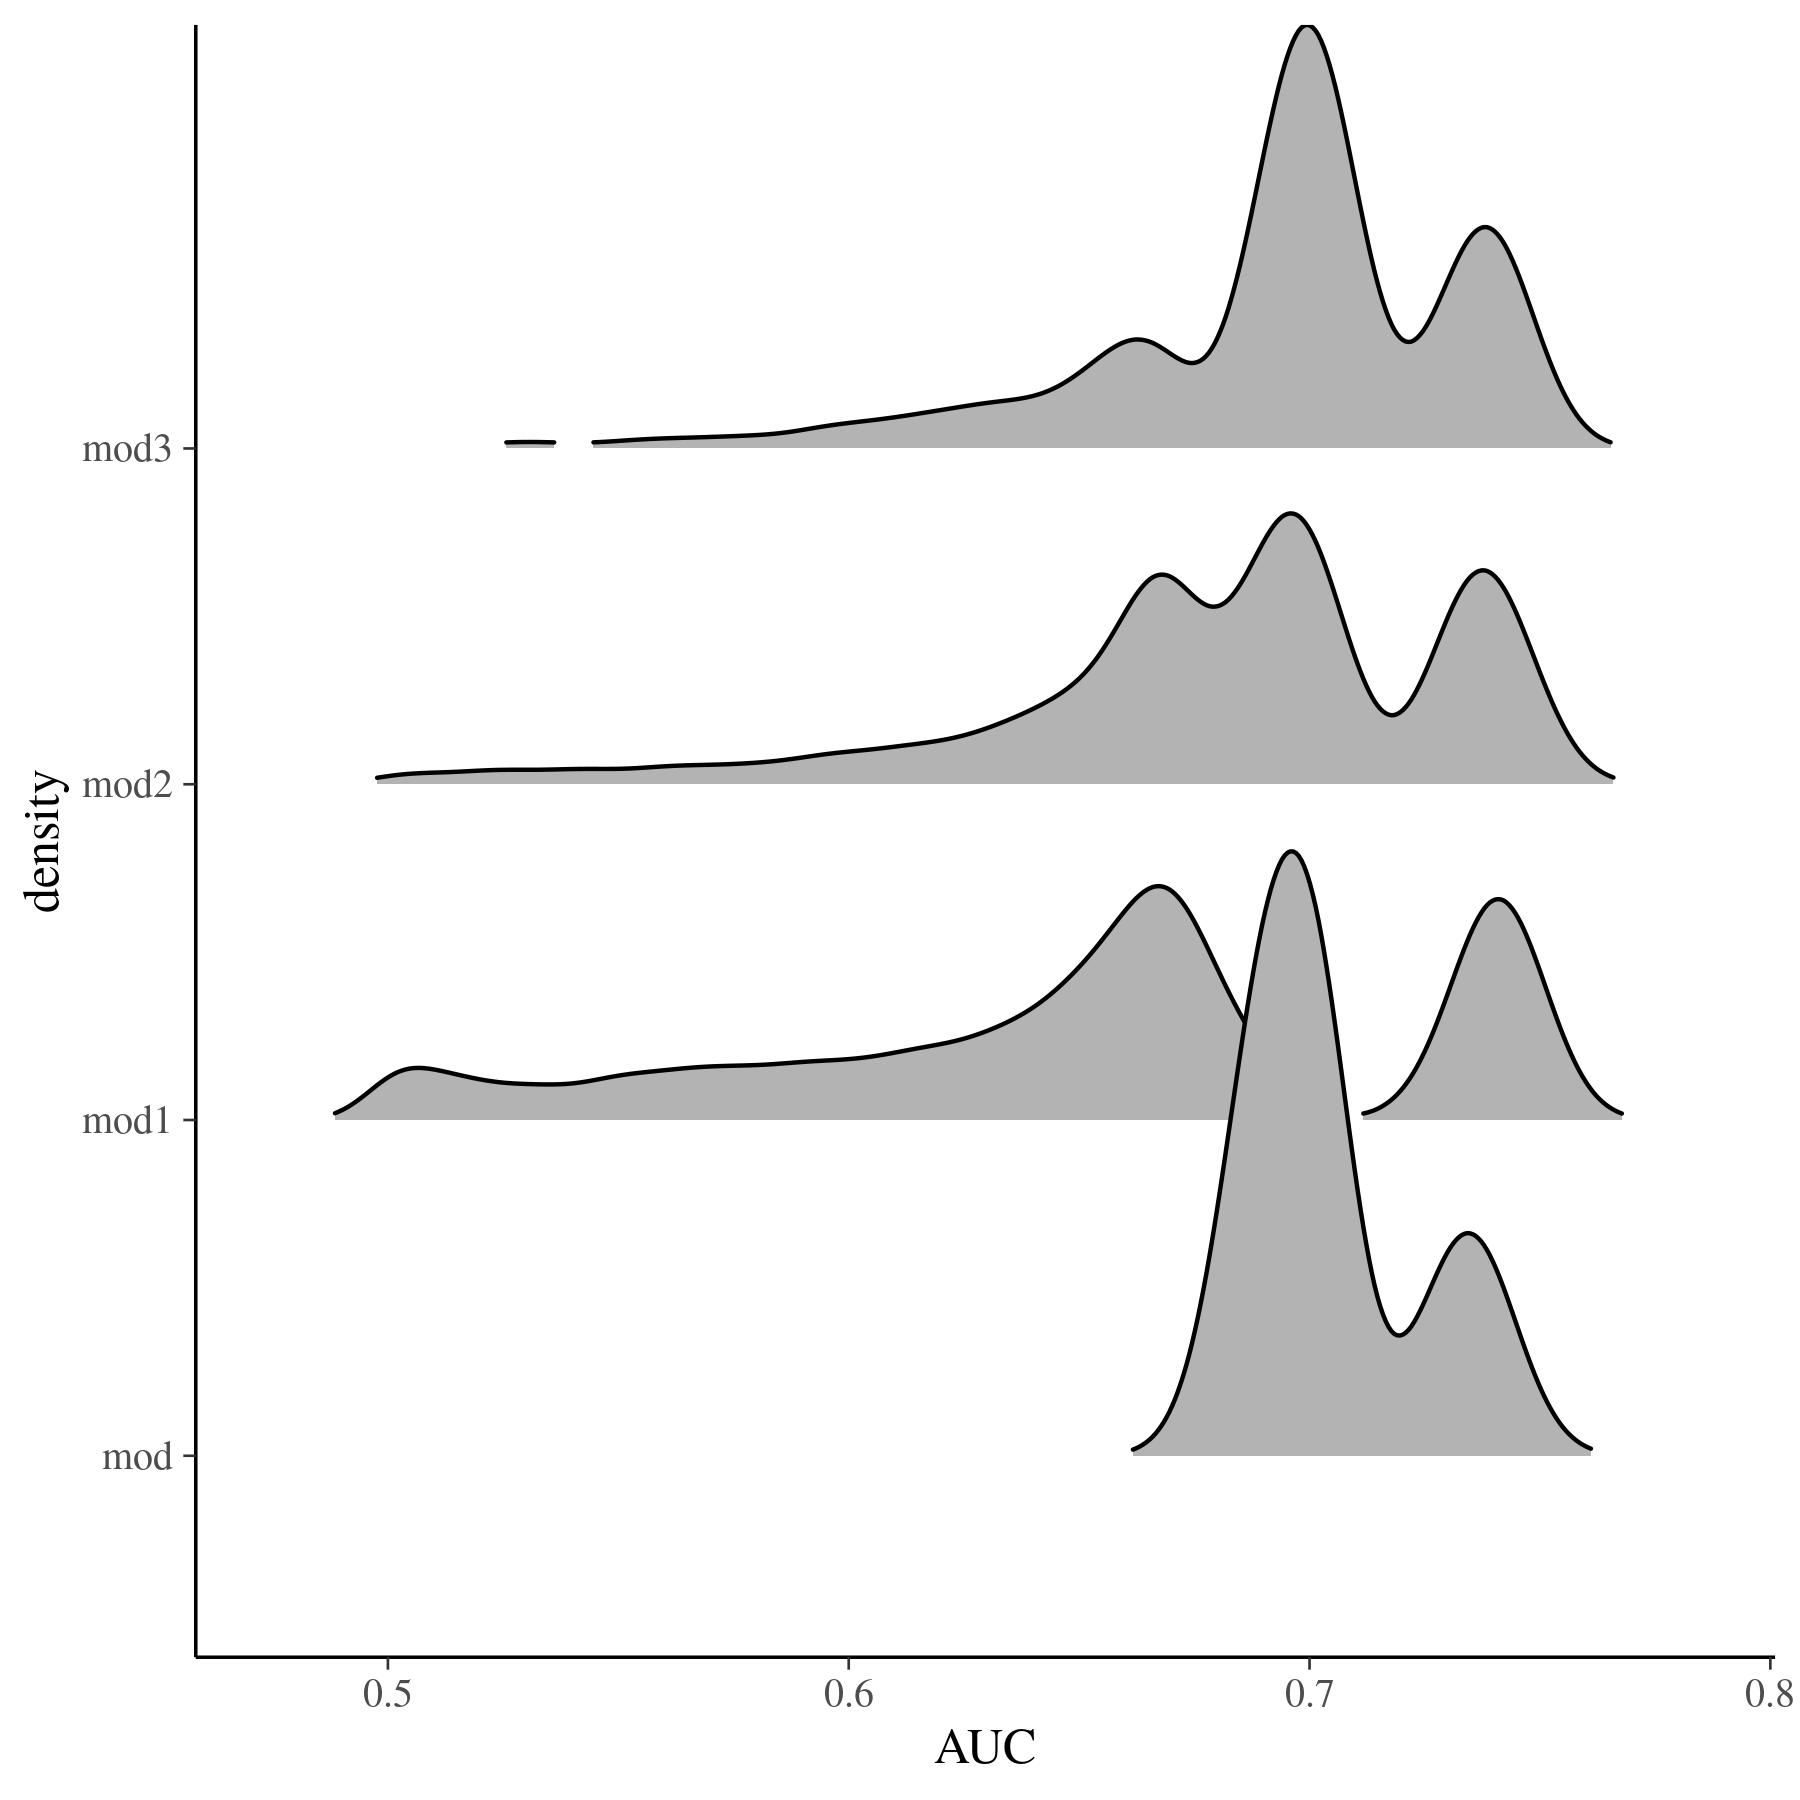
\includegraphics[width=\textwidth,height=0.8\textheight,keepaspectratio=true]{../results/figure/fold_auc}

\end{frame}


\begin{frame}
  \frametitle{Cross-validation results, by time}

  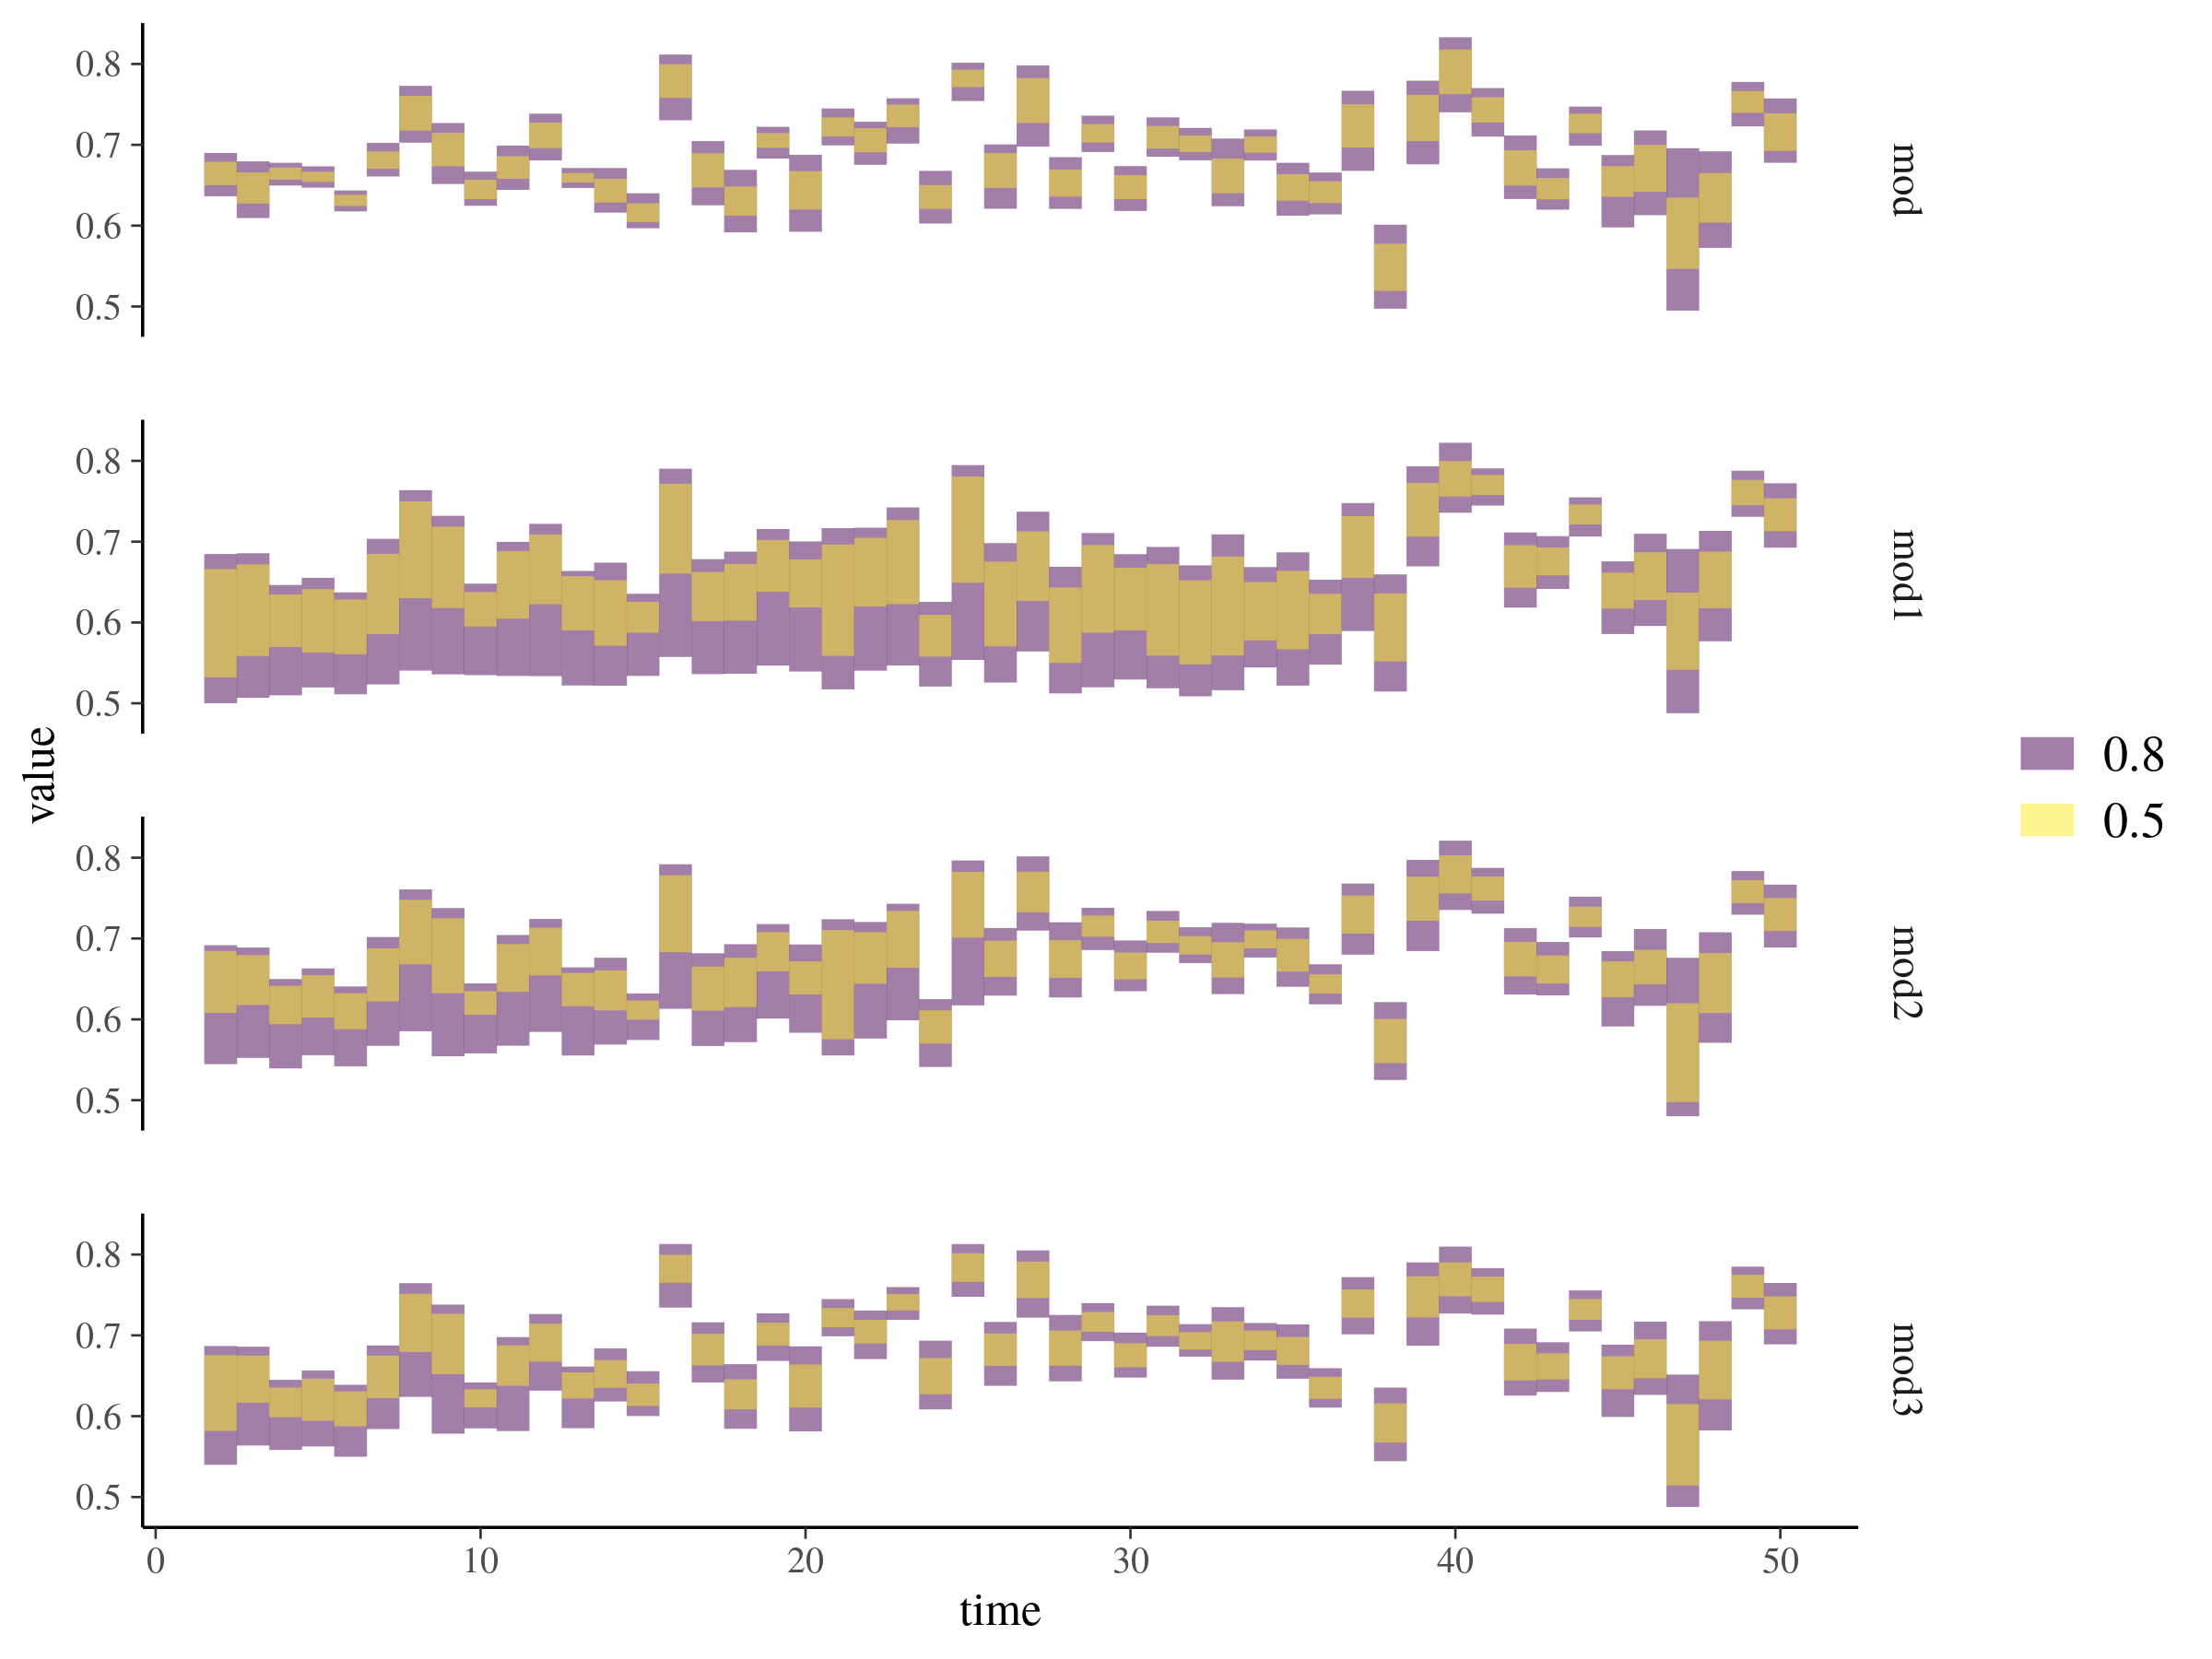
\includegraphics[width=\textwidth,height=0.8\textheight,keepaspectratio=true]{../results/figure/fold_auc_time}

\end{frame}


\begin{frame}
  \frametitle{Summary}

\end{frame}


\begin{frame}
  \frametitle{Conclusions}

\end{frame}


\begin{frame}
  \frametitle{Acknowledgements}

\end{frame}



\appendix

% move to back
\begin{frame}
  \frametitle{A statistical model for predicting extinction}

  \begin{equation}
    \begin{aligned}
      t_{i} &\sim \text{Bernoulli}(\Theta) \\
      \Theta_{i} &= \text{logit}^{-1} (X_{i} B_{w[i], p[i]} + A_{d[i], p[i]}) \\
      B_{w, p} &\sim MVN(\alpha_{p}, \Sigma_{B}) \\
      \alpha_{p} &\sim MVN(\mu, \Sigma_{\alpha}) \\
    % double check this\dots is A MVN dist?
      A_{w, p} &\sim MVN(\delta_{p}, \Sigma_{A}) \\
      \delta_{p} &\sim \mathrm{N}(0, \sigma_{\delta}) \\
      \mu_{d} &\sim 
      \begin{cases}
        N(0, 10) & \text{if } d = 1 \\
        N(-1, 3) & \text{if } d = 2 \\
        N(0, 3) & \text{if } d > 2 \\
      \end{cases}
      \Sigma_{B} &= diag(\tau_{B}) \Omega_{B} diag(\tau_{B}) \\
      \Sigma_{\alpha} &= diag(\tau_{\alpha}) \Omega_{\alpha} diag(\tau_{\alpha}) \\
      \Sigma_{A} &= diag(\tau_{A}) \Omega_{A} diag(\tau_{A}) \\
      \tau_{B} &\sim C^{+}(5) \\
      \tau_{\alpha} &\sim C^{+}(5) \\
      \tau_{A} &\sim C^{+}(5) \\
      \Omega_{B} &\sim LKJ(1) \\
      \Omega_{\alpha} &\sim LKJ(1) \\
      \Omega_{A} &\sim LKJ(1) \\
    \end{aligned}
  \end{equation}

\end{frame}


\begin{frame}
  \frametitle{Effects of age on extinction risk, by phylum}

  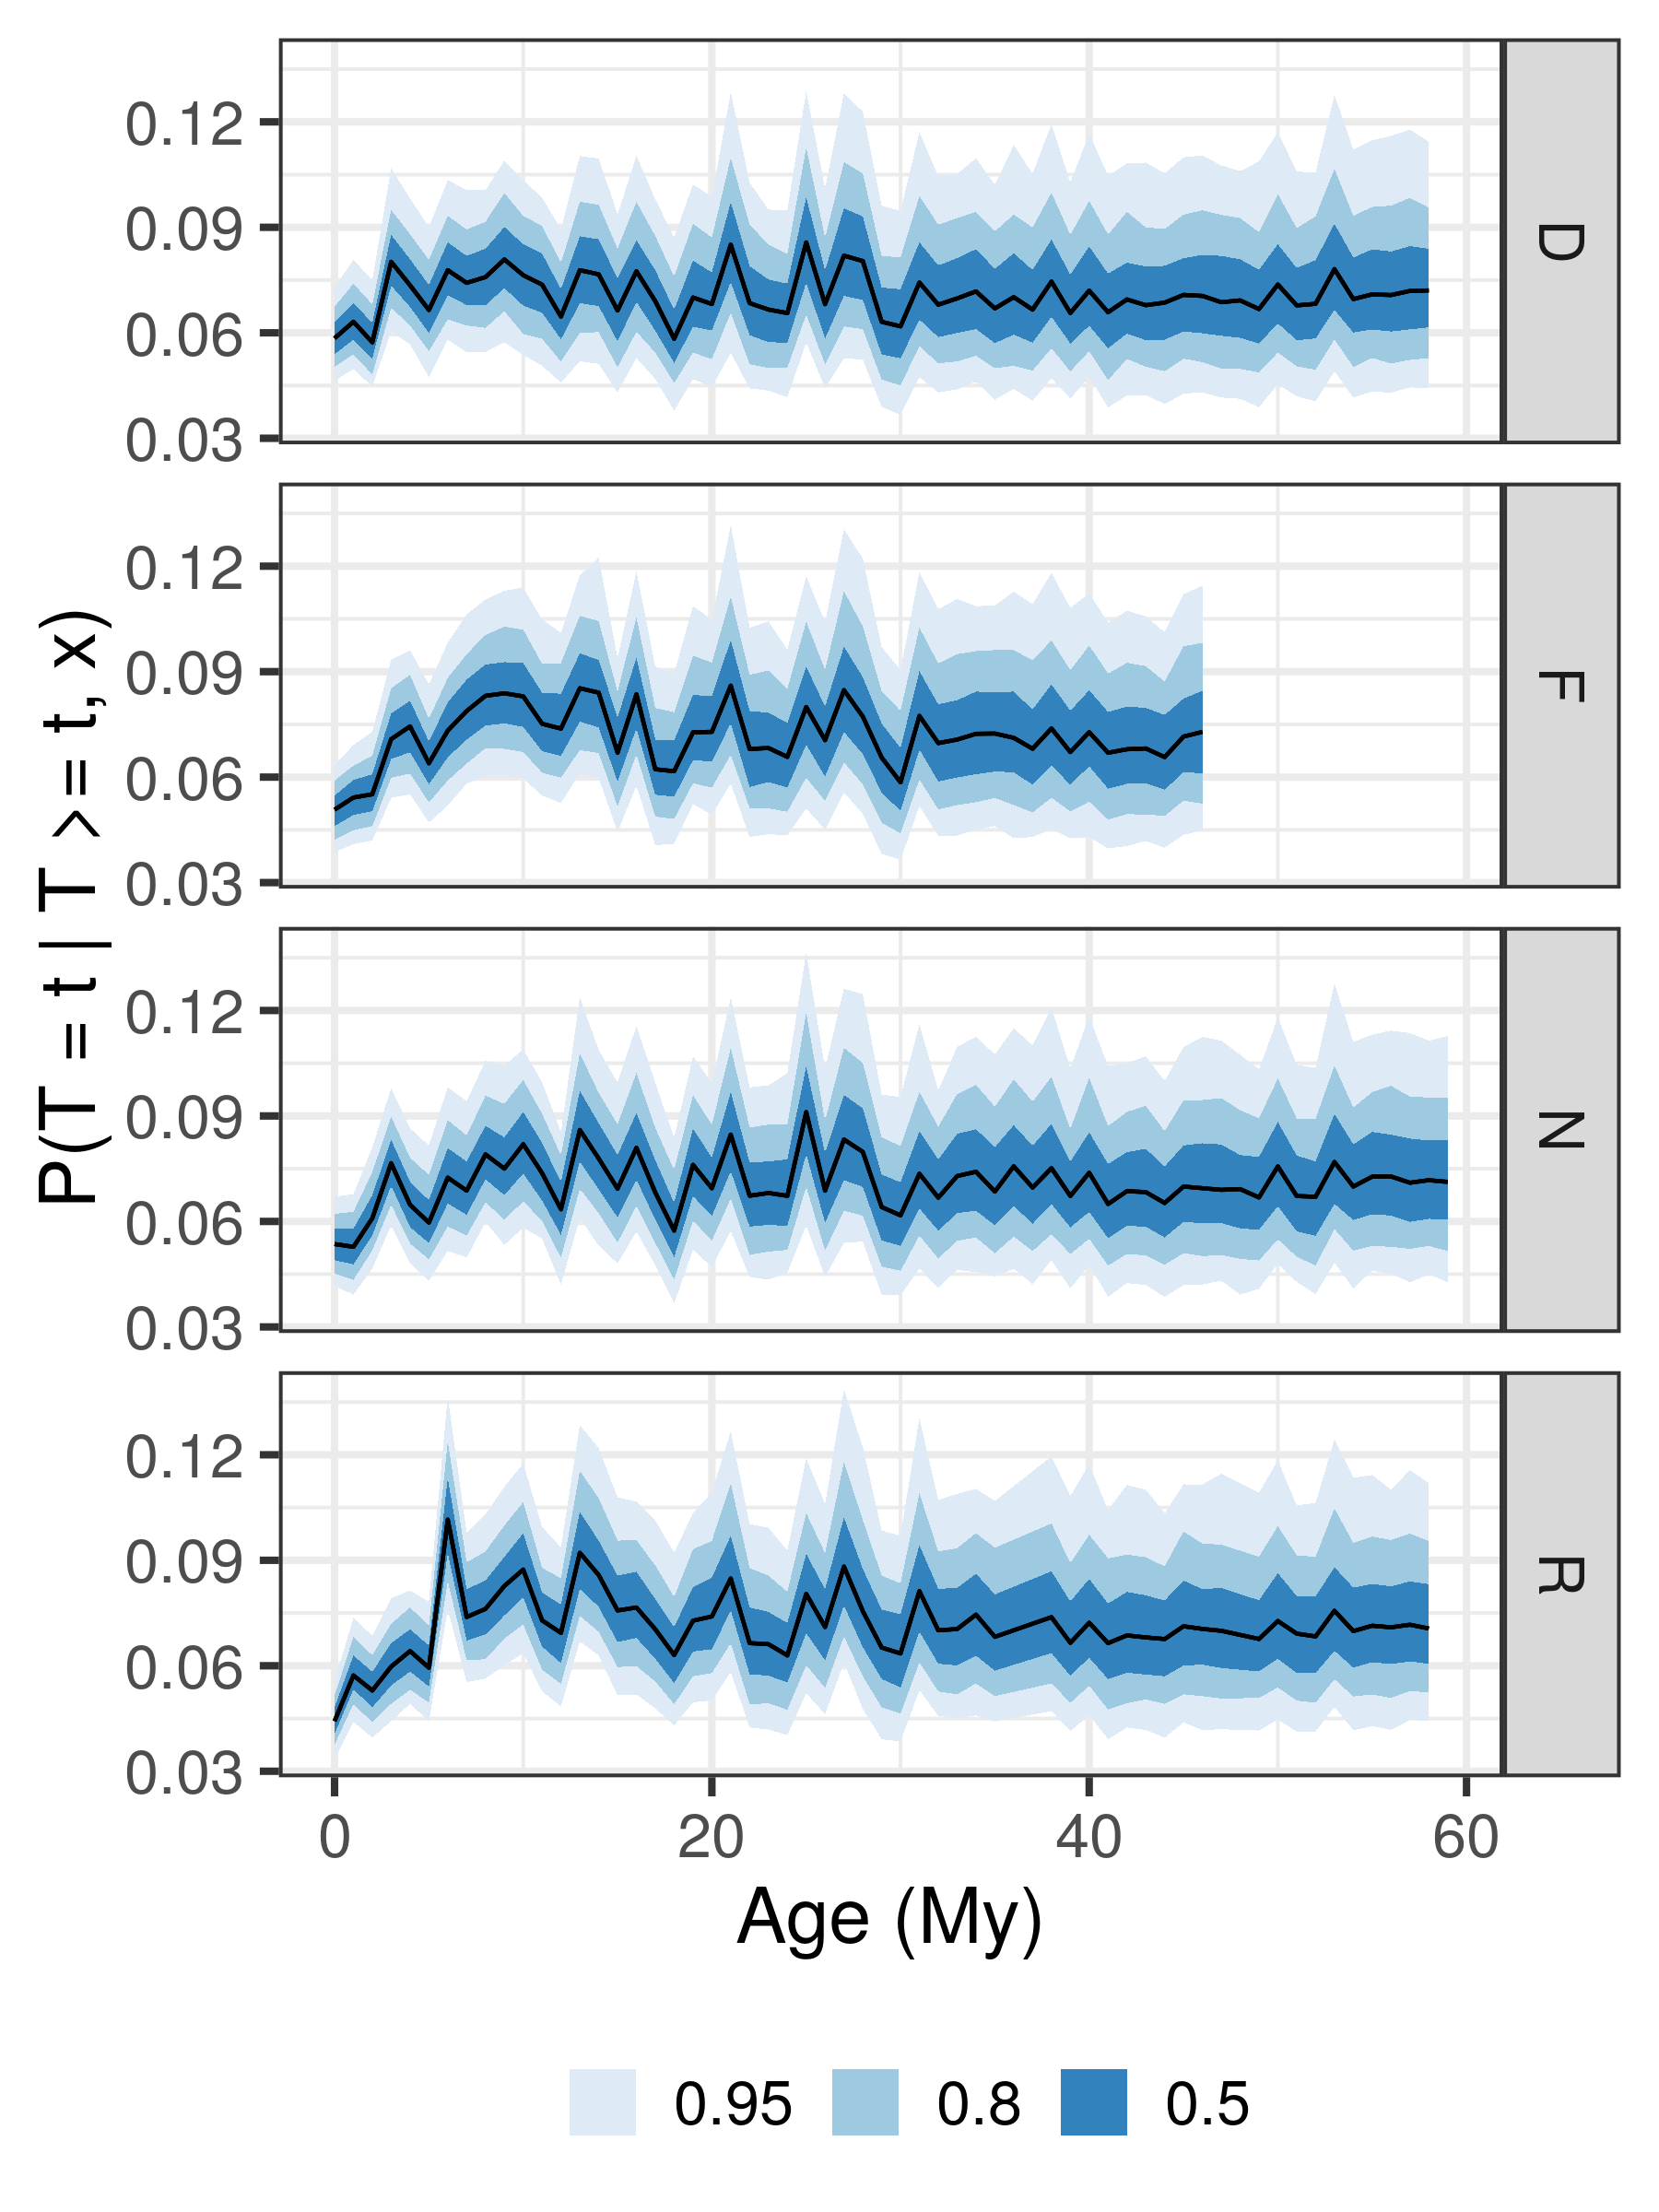
\includegraphics[width=\textwidth,height=0.8\textheight,keepaspectratio=true]{../results/figure/hazard_bygroup}

\end{frame}

\end{document}
